\documentclass[12pt, a4paper]{article}
\usepackage[top=1.0in, bottom=1.0in, left=0.8in, right=0.8in]{geometry}

\setlength{\parskip}{\baselineskip}%
\setlength{\parindent}{0pt}%
\usepackage{bookmark}
\usepackage[]{graphicx}
\usepackage{enumitem}
\usepackage{amsmath}
\usepackage{relsize}
\usepackage{cprotect}
\usepackage{amsmath, amsfonts}
\usepackage{siunitx}
\usepackage{mathrsfs}
\usepackage{framed}
\usepackage{enumitem}
\usepackage{tikz}
\usepackage{circuitikz}
\usepackage{float}
\usepackage[english]{babel}
\usepackage{blindtext}

\newlist{notes}{enumerate}{1}
\setlist[notes]{label=\textbf{Note:} ,leftmargin=*}

\newlist{hints}{enumerate}{1}
\setlist[hints]{label=\textbf{Hint:} ,leftmargin=*}

\usepackage{xcolor}
\usepackage{color}
\definecolor{com1}{RGB}{125,125,125}
\definecolor{comment}{RGB}{140,115,115}
\definecolor{numbering}{rgb}{0.2,0.2,0.2}
\definecolor{key}{RGB}{0,0,180}
\definecolor{in}{RGB}{0,100,0}
\definecolor{out}{RGB}{100,30,30}
\definecolor{bg}{RGB}{245,245,245}
\definecolor{bgLight}{RGB}{250,250,250}
\definecolor{string}{RGB}{0,150,0}

\usepackage{hyperref}
\hypersetup{
    colorlinks=true,
    linkcolor=blue,
    filecolor=magenta,      
    urlcolor=blue,
}
\urlstyle{same}

\usepackage{listings}

\lstdefinestyle{py_code}{ %
    backgroundcolor=\color{bg},      % choose the background
    basicstyle=\ttfamily\small,		      % fonts
    breakatwhitespace=false,         % automatic breaks at whitespace ?
    breaklines=true,                 % sets automatic line breaking
    captionpos=b,                    % caption-position - bottom
    commentstyle=\itshape\color{comment},    % comment style
    extendedchars=true,              % use non-ASCII
    frame=single,	                   % single frame around the code
    keepspaces=true,                 % keeps spaces in text
    keywordstyle=\bfseries\color{key},% keyword style
    language=Python,                 	  % the language of the code
    morekeywords={Null},       % add more keywords to the set
    numbers=left,                    % line_numbers (none, left, right)
    numbersep=10pt,                  % line_no - code dist
    numberstyle=\footnotesize\color{numbering}, % line_no style
    rulecolor=\color{black},         % frame_color [!always set]
    showspaces=false,                % show spaces everywhere
    showstringspaces=false,          % 
    showtabs=false,                  % 
    stepnumber=1,                    % step b/w two line-no
    stringstyle=\color{string},     % string literal style
    tabsize=2,	                       % sets default tabsize to 2 spaces
    title=\lstname,                  % show the filename
    escapeinside={(*}{*)},			  % escape from style inside (* *)
    xleftmargin=\parindent,
    belowskip=-1.3 \baselineskip,
    aboveskip=1.0 \baselineskip,
    columns=fullflexible,
    xleftmargin=0.15in,
}
\lstnewenvironment{py_code}
{\lstset{style=py_code}}
{}

\lstdefinestyle{psudo}{ %
    backgroundcolor=\color{bgLight},   % choose the background
    basicstyle=\ttfamily\small,		      % fonts
    breakatwhitespace=false,         % automatic breaks at whitespace ?
    breaklines=true,                 % sets automatic line breaking
    captionpos=b,                    % caption-position - bottom
    commentstyle=\itshape\color{com1},          % comment style
    extendedchars=true,              % use non-ASCII
    keepspaces=true,                 % keeps spaces in text
    language=C,                 	  % the language of the code
    morekeywords={type,NULL, True, False},       % add more keywords to the set
    showspaces=false,                % show spaces everywhere
    showstringspaces=false,          % 
    showtabs=false,                  % 
    tabsize=2,	                       % sets default tabsize to 2 spaces
    title=\lstname,                  % show the filename
    escapeinside={(*}{*)},			  % escape from style inside (* *)
    belowskip=-1.8 \baselineskip,
    aboveskip=0.9 \baselineskip,
    columns=fullflexible,
    xleftmargin=0.2in,
    frame=tb,
    framexleftmargin=16pt,
    framextopmargin=6pt,
    framexbottommargin=6pt, 
    framerule=0pt,
}

\lstnewenvironment{psudo}
{\lstset{style=psudo}}
{}

\graphicspath{ ./ }

\title{\textbf{EE2703 : Applied Programming Lab \\ Assignment 8 \\ Discrete Fourier Transform}} 
\author{Chagari Koushal Kumar Reddy \\ EE20B023} % Author name

\date{\today} % Date for the report

\begin{document}		

\maketitle % Insert the title, author and date
\clearpage

\tableofcontents
\clearpage

\section{Aim}
The aim of this assignment is to:
\begin{enumerate}
    \item Learn Digital Fourier Transform (DFT) and it's properties.
    \item Use the in-built Python library to generate DFT of various discrete time signals using the Fast Fourier Transform (FFT) algorithm.
    \item Analyze the continuous time Fourier Transform (CTFT) of continuous time signals by plotting the DFT of their sampled DT versions.
\end{enumerate}
\section{Theory}
\subsection{Sampling}
Sampling is an important concept in digital signal processing. It is the process of creating a discrete-time signal from a known continuous time signal by sampling it
at regular intervals. Also all digital devices and computers we use can perform arithmetic and algorithmic analysis only on discrete data. Hence sampling is a very important concept in signal processing.

Let's say the CT signal is $x_{c}(t)$. Now the sampled DT signal will be:
\begin{equation*}
    x[n] = x_{c}(t)|_{t=nT_{s}} = x_{c}(nT_{s})
\end{equation*}
where $T_{s}$ is the sampling period. The associated sampling frequency is:
\begin{equation*}
    \Omega_{s} = \frac{2\pi}{T_{s}}
\end{equation*}
\subsection{Nyquist-Shannon Sampling Theorem}
Whenever we sample a CT signal $x_{c}(t)$ and obtain a DT signal $x[n]$, their spectra: $X_{c}(\Omega)$ and $X(\omega)$ are related as:
\begin{equation*}
    X(\omega) = \frac{1}{T_{s}} \sum_{k=-\infty}^{\infty} X_{c}(\frac{\omega}{T_{s}}-k\frac{2\pi}{T_{s}})
\end{equation*}
Now the Nyquist-Shannon sampling theorem states that for a bandlimited signal $x_{c}(t)$, the sampling frequency $\Omega_{s}$ should be atleast twice the maximum frequency present in the spectrum of $x_{c}(t)$ in order to prevent overlapping (or Aliasing).
Only if this condition is satisfied, the DTFT of $x[n]$ will preserve the original information about the CT signal.
\subsection{Discrete Fourier Transform (DFT)}
Discrete Fourier Transform (DFT) is an important concept in digital signal processing. As we already saw, we have a continuous variable spectrum pertaining to DT signals known as the Discrete-Time Fourier Transform (DTFT) which is given by:
\begin{equation*}
    X(\omega) = \sum_{n=-\infty}^{\infty}x[n]e^{-j\omega n}
\end{equation*}
This is a real variable function and is defined for a continuum of values. DFT, on the other hand is a discrete variable signal and is defined only for certain integer values. Let's assume we have an N-periodic DT signal, i.e., if we know its first N samples ($x[0], x[1], \ldots , x[N-1]$), we know the full signal. Now its DTFT is also periodic with period as N samples and is defined as:
\begin{equation*}
    a[k] = \sum_{n=0}^{N-1}x[n]e^{-j \frac{2\pi}{N} kn}
\end{equation*}
\begin{equation*}
    x[n] = \sum_{k=0}^{N-1}\frac{a[k]}{N}e^{j \frac{2\pi}{N} kn}
\end{equation*}
and both k and n belong to the set $0,1,2,\ldots, N-1$. Also, the DT signal $x[n]$ calculated by the inverse DFT formula is inherently periodic with period of N samples. Hence DFT is usually used to analyze periodic DT signals. Their values present in one single period contains all information about that signal and its DFT. Note that both $x[n]$ and its DFT $a[k]$ are periodic with period as 'N' samples.
\subsection{Connection between CTFT and DFT}
Let's say we have a finite length CT signal and this signal, when periodically extended and sampled, gives us a DT signal. Let us define the following functions:
\begin{enumerate}
    \item $x(t)$ = Finite length CT signal of length $T_{o}$
    \item $X_{fin}(\Omega)$ = CTFT of x(t)
    \item $x_{c}(t)$ = Periodic extension of $x(t)$ with period $T_{o}$
    \item $\Omega_{o}$ = Fundamental frequency of $x_{c}(t) = \frac{2pi}{T_{o}}$
    \item $a_{k}$ = $k^{th}$ CTFS coefficient of $x_c(t)$
    \item $X_c{\Omega}$ = CTFT of periodic CT signal $x_c(t)$
    \item $x[n]$ = Sampled version of $x_{c}(t)$, i.e., $x_{c}(nT_{s})$
    \item $\Omega_{s}$ = Sampling frequency = $\frac{2pi}{T_{s}}$
    \item $\omega_{o}$ = DFT resolution frequency = $\frac{2pi}{N}$
    \item $X(\omega)$ = DTFT of the signal $x[n]$
    \item $a[k] = k^{th}$ DFT coefficient of signal $x[n]$ 
\end{enumerate}
Let's assume the first N samples that define x[n] are given by sampling the $T_{o}$ period signal $x(t)$. Hence $T_{s} = \frac{T_{o}}{N}$. We have the following important equations which relate the spectra of CT signal and the sampled DT signal:
\begin{equation}
    X_{fin}(k\Omega_{o}) = T_{o} a_{k}
\end{equation}
\begin{equation}
    X_{c}{\Omega} = \sum_{k=-\infty}^{\infty}2\pi a_{k}\delta(\Omega-k\Omega_{o})
\end{equation}
\begin{equation}
    X(\omega) = \frac{1}{T_{s}} \sum_{k=-\infty}^{\infty}X_{c}(\frac{\omega}{T_{s}}-k\frac{2\pi}{T_{s}})
\end{equation}
\begin{equation}
    X(\omega) = \sum_{k=0}^{N-1} \frac{2\pi a[k]}{N}\delta (\omega -k\omega _{o})
\end{equation}
The last equation relates the DTFT and DFT of periodic DT signal x[n]. Now let's assume that the CTFT of the periodic CT signal $x_{c}(t)$ is bandlimited or atleast has a decreasing trend in the fourier series coefficients such that we can assume that the spectrum is approximately bandlimited after a particular value of $k$.
Now we can choose a sampling frequency $\Omega _{s}$ such that the Nyquist criteria is met, i.e., $\Omega _{s} > 2\Omega _{m}$ where $\Omega _{m}$ is the maximum frequency component present in $X_{c}(\Omega)$.


Any CT frequency $\Omega$ we have will become $\Omega T_{s}$ in the DT domain. Hence a frequency of $\frac{\Omega}{2}$ in CT domain becomes $\frac{\Omega T_{s}}{2} = \pi$ in the DT domain. So a range of $-[\frac{-\Omega _{s}}{2}, \frac{\Omega_{s}}{2})$ in the DT domain. Also since the Nyquist criteria is assumed to be satisfied, we can safely say:
\begin{equation}
    X(\omega) = \frac{1}{T_{s}}X_{c}(\frac{\omega}{T_{s}})
\end{equation} 
for $\omega \in [-\pi,\pi)$. We are able to get this equation only because Nyquist criteria is satisfied. Else the shifted spectrum terms will also contribute to $X(\omega)$. With this assumption, let's see how $X(\omega)$ will be related to DFT coefficients. From equation (4),(5), we can say:
\begin{equation}
    X_{c}(\frac{\omega}{T_{s}}) = \sum_{k=0}^{N-1}\frac{2\pi T_{s}a[k]}{N}\delta(\omega - k\omega_{o}) = \sum_{k=-\infty}^{\infty}2\pi a_{k}\delta(\frac{\omega}{T_{s}}-k\frac{2\pi}{T_{o}}) = \sum_{k=-\infty}^{\infty}2\pi T_{s}a_{k}\delta(\omega-k\frac{2\pi}{N})
\end{equation}
Since we have assumed that the CTFS coefficients are limited within $[-\frac{\Omega_{s}}{2},\frac{\Omega_{s}}{2})$ in the CT domain, they will be restricted in $[-\pi,\pi)$ on the DT domain or the $\omega$-axis. So our eqn(6) reduces to:
\begin{equation*}
    \sum_{k=-\frac{N}{2}}^{\frac{N}{2}-1}\frac{2\pi T_{s}a[k]}{N} \delta(\omega - k\omega_{o}) = \sum_{k=-\frac{N}{2}}^{\frac{N}{2}-1}2\pi T_{s}a_{k} \delta(\omega - k\frac{2\pi}{N})
\end{equation*}
Clearly we have:
\begin{equation}
    a_{k} = \frac{a[k]}{N}
\end{equation}
Now also we have:
\begin{equation}
    X_{fin}(k\Omega_{o}) = T_{o}\frac{a[k]}{N} = T_{s}a[k]
\end{equation}
The final takeaway point is that if we can safely assume the signal is bandlimited and the sampling frequency satisfies the Nyquist crieria, then the CTFT of the finite length CT signal $x(t)$ can be computed at integer values of frequency $\Omega_{o}$ by multiplying the N-point DFT of the sampled version by $T_{s}$.
\begin{itemize}
    \item CT frequency interval : $[\frac{-\pi N}{T_{s}},\frac{\pi N}{T_{s}}]$
    \item CT frequency least count: $\Omega_{o} = \frac{2 \pi}{T_{s}}$
\end{itemize}
Hence to get the CTFT for a higher range, we can either increase N or decrease $T_{o}$ or do both. However the resolution can be improved only by increasing $T_{o}$. Hence, when we aim to increase the resolution the range automatically gets shortened. To maintain same range, we need to proportionately increase N.
\section{Assignment}
\subsection{Spectrum of $\sin(5t)$}
Sin($5t$) is a very simple continuous time function. Let's analyze some of its parameters and properties.
\begin{itemize}
    \item Has a single CT frequency of $\Omega = 5$ rad/s.
    \item Spectrum is bandlimited i.e., only two impulses are present at $\Omega = \pm 5$ rad/s.
    \item Since it is periodic, its CTFT will have impulses. So its better to plot its CTFS coefficients 
\end{itemize}
We can write $\sin(5t)$ as:
\begin{equation*}
    \sin(5t) = \frac{e^{j5t}-e^{-j5t}}{2j} = -0.5je^{j5t} + 0.5je^{-j5t}
\end{equation*}
Clearly the CTFS coefficients are $-0.5$j and $0.5$j. To get this plot using DFT of the sampled version, we need to satisfy the Nyquist creiteria. Also, for the Fast Fourier Transform (FFT) algorithm to work faster, we need to choose an N which a power of 2. Hence let's choose $N=128$. Also let the finite length signal whose periodic representation is $\sin(5t)$ have a length of $2\pi$ i.e., it is $\sin(5t)$ for $t \in [0,2\pi)$ and zero outside. Hence $T_{o} = 2\pi$. Thus, $T_{s}=\frac{2\pi}{128}$ and $\Omega_{s}=128$. Clearly $128>2*5=10$. Hence Nyquist criteria is also satisfied. Now, we have:
\begin{equation*}
    a_{k} = \frac{a[k]}{N}
\end{equation*}
So in our code, after finding the DFT coefficients, we should divide the vector by $N$ to get the CTFS coefficients. after doing all that and plotting tha magnitude and phase response plots, we have the following plot:
\vspace*{-0.5cm}
\begin{figure}[H]
    \centering
    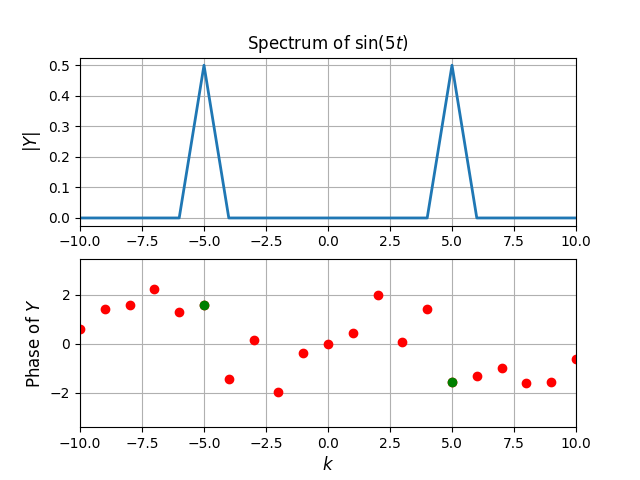
\includegraphics[scale = 0.8]{Figure_1.png}
    \label{fig:sample}
\end{figure}
\begin{center}
    There are peaks of length $0.5$ at $\Omega_{o} = \pm5$ as expected
\end{center}
The phase at $\frac{\pi}{2}$ at $\Omega_{o}=-5$ and $\frac{\pi}{2}$ at $\Omega_{o}=5$ as expected. Hence, the plot is correct. To get a more precise plot, we need to increase $T_{o}$ as resolution will increase but at the same time, we should increase $N$ to maintain the same frequency range for which the CTFT (or CTFS) is calculated. The plot given is for $N=1024$ and $T_{o}=8\pi$:

\begin{figure}[H]
    \centering
    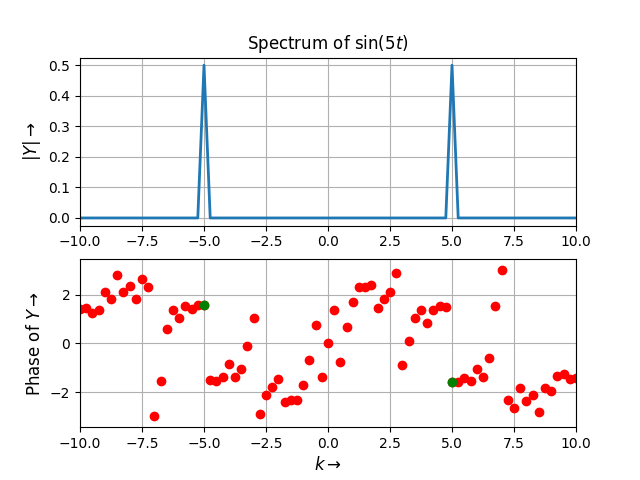
\includegraphics[scale = 0.8]{Figure_2.png}
    \label{fig:sample}
\end{figure}
\begin{center}
    A much better plot with higher resolution
\end{center}
\subsection{Spectrum of amplitude modulated signal}
AM modulation is a common technique used in communication of signals. A signal which is to be tranmistted, will be modulated over a carrier frequency so that the modulated signal can be transmistted using antennas of small length. The modulated signal can again be converted back to the original signal using signal processing techniques on the receiver end. Let us consider the following example:
\begin{equation*}
    x(t) = (1+0.1\cos(t))\cos(10t)
\end{equation*}
The properties of this signal are:
\begin{itemize}
    \item Has 3 CT frequencies at $\Omega = 9,10,11$ rad/s.
    \item Spectrum is bandlimited i.e., only 2 impulses are present at $\Omega = \pm 9,\pm 10, \pm 11$ rad/s.
    \item Since it is periodic, its CTFT will have impulses. So its better to plot its CTFS coefficients
\end{itemize}
We can write this signal as:
\begin{equation*}
    x(t) = 0.025e^{j9t} + 0.025e^{-j9t} + 0.5e^{j10t} + 0.5e^{j10t} + 0.025e^{j11t} + 0.025e^{-j11t}
\end{equation*}
In this question, let's assume we choose $T_{o}=2\pi$ and $N=128$. Now the least count is $\Omega_{o} = \frac{2\pi}{T_{o}} = 1$ rad/s. And the CT frequencies we have also differ by $1$ rad/s. Hence when we plt, we won't get distinct impulses. We will get an interpolated plot which is wrong. The plot is given below:
\vspace*{-0.5cm}
\begin{figure}[H]
    \centering
    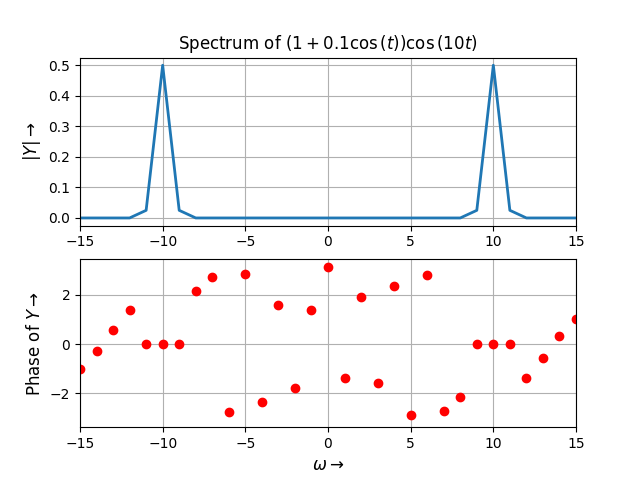
\includegraphics[scale = 0.8]{Figure_3.png}
    \label{fig:sample}
\end{figure}
\begin{center}
    We get interpolated plot which is not correct
\end{center}
To resolve this problem, we need to set the least count less than 1. Our previous least count was $\Omega_{o} = \frac{2\pi}{T_{o}} = 1$ rad/s. Now, let's say $T_{o} = 8\pi$ and $N=1024$. Now the new least count is $\Omega_{o} = \frac{2\pi}{T_{o}} = 0.25$ rad/s. Clearly, now we won't have any wrong interpolation and the graph will be much better and visually appealing. The plot is as given below:
\vspace*{-0.5cm}
\begin{figure}[H]
    \centering
    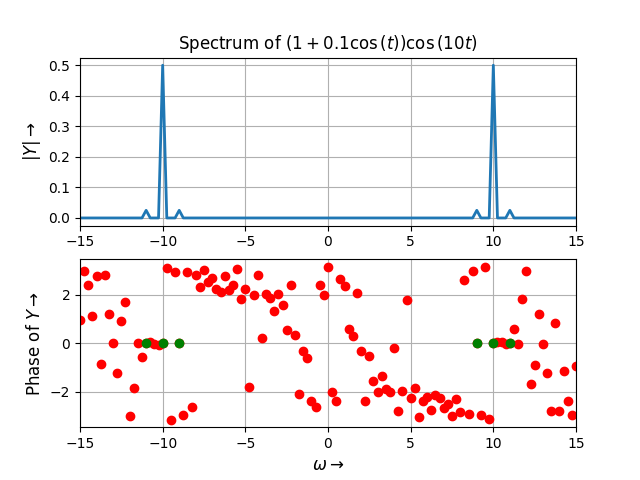
\includegraphics[scale = 0.8]{Figure_4.png}
    \label{fig:sample}
\end{figure}
\begin{center}
    The plot contains magnitudes which are exactly same as the mathematical results we got and the phases are also zero at those frequencies
\end{center}
\subsection{Spectrum of $\sin^{3}(t), \cos^{3}(t)$}
Both signals $\sin^{3}(t)$ and $\cos^{3}(t)$ are periodic with bandlimited spectrum. We can write them as:
\begin{equation*}
    \sin^{3}(t) = \frac{3}{4}\sin(t) - \frac{1}{4}\sin(3t) = -0.375je^{jt} + 0.375je^{-jt} + 0.125je^{j3t} - 0.125je^{-j3t}
\end{equation*}
\begin{equation*}
    \cos^{3}(t) = \frac{3}{4}\cos(t) + \frac{1}{4}\cos(3t) = 0.375je^{jt} + 0.375je^{-jt} + 0.125je^{j3t} + 0.125je^{-j3t}    
\end{equation*}
Hence the spectrum of both the signals will contain distinct impulses at frequencies 1 and 3 rad/s. The plots are given below:
\vspace*{-0.5cm}
\begin{figure}[H]
    \centering
    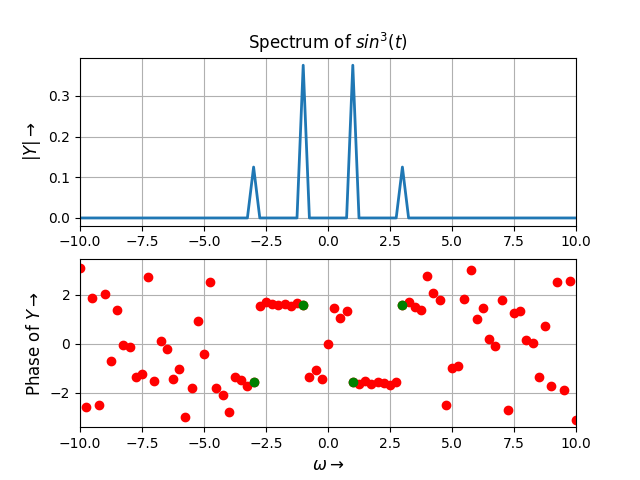
\includegraphics[scale = 0.8]{Figure_5.png}
    \label{fig:sample}
\end{figure}
\begin{center}
    As expected we have peaks of lengths 0.375 and 0.125. Also, we have phases as $-\frac{\pi}{2}$ and $\frac{\pi}{2}$ at the correct frequencies
\end{center}
\vspace*{-0.5cm}
\begin{figure}[H]
    \centering
    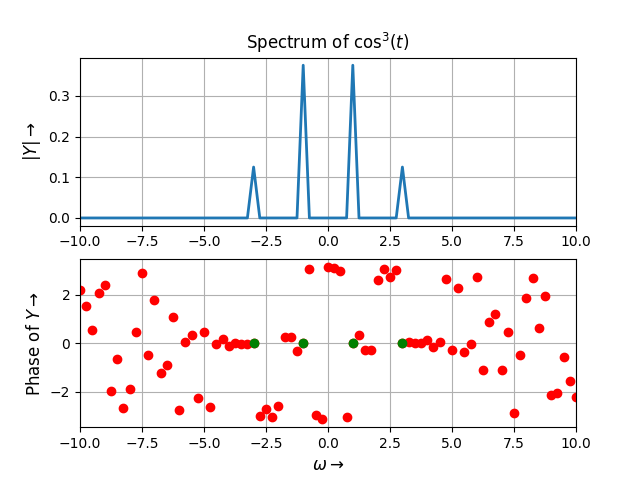
\includegraphics[scale = 0.8]{Figure_6.png}
    \label{fig:sample}
\end{figure}
\begin{center}
    Similar to previous graph, we have peaks of lengths 0.375 and 0.125. However, now the phases are purely 0 as expected
\end{center}
\subsection{Spectrum of frequency modulated signal}
\textbf{Note:} Only in this section, both $\Omega$ and $\omega$ denote CT frequencies.

Sometimes, signals are also frequency modulated before tranmsission. One such example is:
\begin{equation*}
    x(t) = \cos(20t+5\cos(t))
\end{equation*}
We can write this function as a sum of complex exponentials based on \textbf{Laurent's expansion of Bessel's function}.
\begin{equation*}
    exp(\frac{\beta}{2}(z-\frac{1}{z})) = \sum_{k=-\infty}^{\infty}J_{k}(\beta)z^{k}
\end{equation*}
Substituting $z = jexp(jw_{m}t)$, we have:
\begin{equation*}
    exp(j\beta\cos(w_{m}t)) = \sum_{k=-\infty}^{\infty}J_{k}(\beta)j^{k}exp(jkw_{m}t)
\end{equation*}
Now we have:
\begin{equation*}
    \cos(w_{c}t+\beta\cos(w_{m}t)) = Re[exp(jw_{c}t+j\beta\cos(w_{m}t))] = Re[e^{jw_{c}t}\sum_{k=-\infty}^{\infty}J_{k}(\beta)e^{j(w_{m}t+\frac{\pi}{2})k}]
\end{equation*}

\begin{equation*}
    \cos(w_{c}t + \beta \cos(w_{m}t)) = \sum_{k=-\infty}^{\infty}J_{k}(\beta)\cos(w_{c}t+kw_{m}t+k\frac{\pi}{2})
\end{equation*}
Writing this as a sum of sinusoids, we have:
\begin{equation*}
    \cos(w_{c}t + \beta \cos(w_{m}t)) = \sum_{k=-\infty}^{\infty}\frac{J_{k}(\beta)}{2}e^{j(w_{c}t+kw_{m}t+k\frac{\pi}{2})} + \sum_{k=-\infty}^{\infty}\frac{J_{k}(\beta)}{2}e^{-j(w_{c}t+kw_{m}t+k\frac{\pi}{2})}
\end{equation*}
Hence when we plot the CTFT, we will have impulses of length $\frac{J_{k}(\beta)}{2}$ centerd around $w_{c}$ and $-w_{c}$. Also the phase of the impulses will depend on the $k$ value. The fourier coefficients i.e., $\frac{J_{k}(\beta)}{2}j^{k}$ are plotted for $\beta=5$ and $w_{m}=1$ as given in the question.
\vspace*{-0.5cm}
\begin{figure}[H]
    \centering
    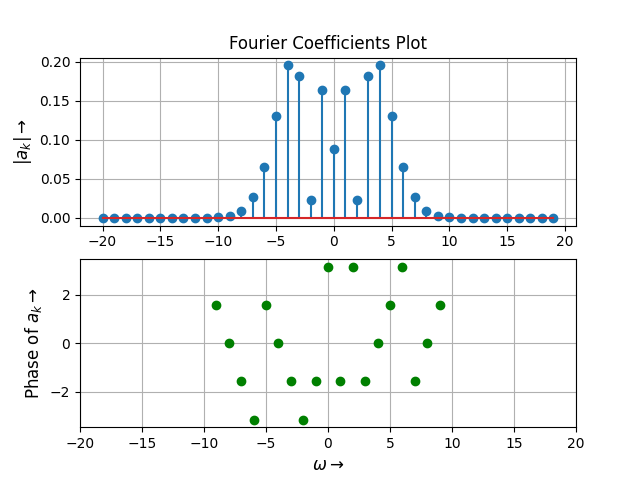
\includegraphics[scale = 0.8]{Figure_7.png}
    \label{fig:sample}
\end{figure}
Now we have an idea about the fourier coefficients of the FM signal. We see that the signal has a bandlimited spectrum with the maximum frequency at $w = \pm 10$ rad/s. So in order to prevent aliasing, we just need to choose a sufficient $N$. Let's assume $T_{o}=32\pi$ and $N=4096$. Hence maximum frequency is $\frac{\Omega}{2}=4096\frac{\pi}{32\pi} = 128 > (20+10) = 30$. Hence we can safely assume that the Nyquist criteria is satisfied. We considered $20 + 10$ and not just $10$ since now, the impulses will be around $w_{c}=10$. Hence, we need to check whether $w_{c}+10$ is less than $\frac{\Omega}{2}$.
\vspace*{-0.5cm}
\begin{figure}[H]
    \centering
    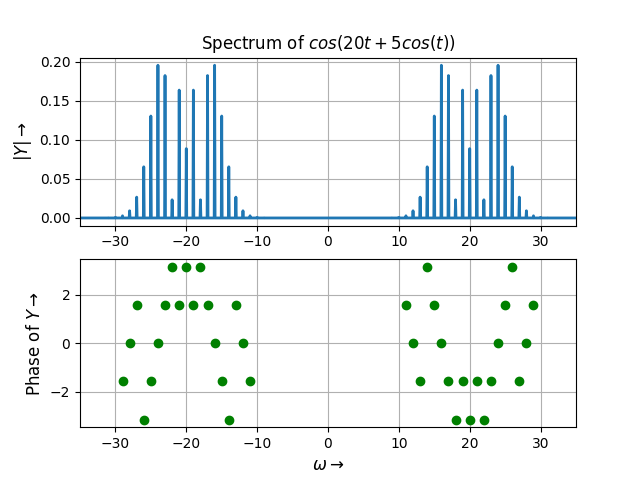
\includegraphics[scale = 0.8]{Figure_8.png}
    \label{fig:sample}
\end{figure}
\begin{center}
    We have peaks at frequency $\Omega = 20 $ and a few frequencies surrounding it. Also the magnitude response is even and the phase response is odd since the CT signal is real.
\end{center}
The plot obtained from the DFT exactly matches the Bessel's function plot generated manually. Hence, the DFT gave an accurate plot of the CTFS of the FM signal.

\textbf{Note:} The theory about CTFS of FM modulated signal and the relation with Bessel's functions was referred from this link: \url{https://www.dsprelated.com/freebooks/mdft/Sinusoidal_Frequency_Modulation_FM.html} 
\subsection{Spectrum of the Gaussian signal}
This Gaussian function is a special signal. Unlike the previous signals, this is a non-periodic signal and also the spectrum is not bandlimited. This is because Gaussian is a \textbf{self-function} i.e., it is it's own fourier transform.

Let the signal be of the form:
\begin{equation*}
    x(t) = e^{-\frac{t^{2}}{2\sigma^{2}}}
\end{equation*}
Then the continuous time fourier tranform of this signal will be:
\begin{equation*}
    X(\Omega) = \sqrt{2\pi\sigma^{2}}e^{-\frac{\Omega^{2}\sigma^{2}}{2}}
\end{equation*}
In the example given in this assignment, $\sigma=1$. Hence the expected plot should be:
\begin{equation*}
    X(\Omega) = \sqrt{2\pi}e^{-\frac{\Omega^{2}}{2}}
\end{equation*}
Now before proceeding forward, we must first analyze some important properties of the signal and makek some valid approximations based on that. The following properties are important:
\begin{itemize}
    \item It is not a bandlimited signal - Satisfying Nyquist criteria exactly is impossible
    \item It is a non-periodic signal
    \item It is a steeply decreasing positive even function and almost looks like a finite length signal
\end{itemize}
Since the guassian is a non-periodic signal, it's CTFT won't necessarily have impulses (Infacr it doesn't have any as we have already derived it's CTFT). So, in order to apply the DFT concepts on it, we must first make a periodic CT signal out of it and sample it. Let's first define a new finite length signal like this:

\begin{equation*}
    x_{finite}(t) = exp(-\frac{t^{2}}{2}) , t\in [-\frac{T_{o}}{2},\frac{T_{o}}{2})
\end{equation*}
and the signal is zero outside this interval. This new function is not the same gaussian function but a finite piece (or window) of it is taken. Now, let's find its CTFT:
\begin{equation*}
    X(\Omega) = \int_{-\infty}^{\infty} exp(-\frac{t^{2}}{2})exp(-j\Omega t)dt \approx \int_{\frac{T_{o}}{2}}^{\frac{T_{o}}{2}} exp(-\frac{t^{2}}{2})exp(-j\Omega t)dt
\end{equation*}
Hence the CTFT of the new finite length function is approximately equal to the CTFT of the Gaussian function. \textbf{This is the first assumption}. Now this signal is periodically repeated and a new periodic signal $x_{c}(t)$ is generated and sampled.
\vspace*{-0.5cm}
\begin{figure}[H]
    \centering
    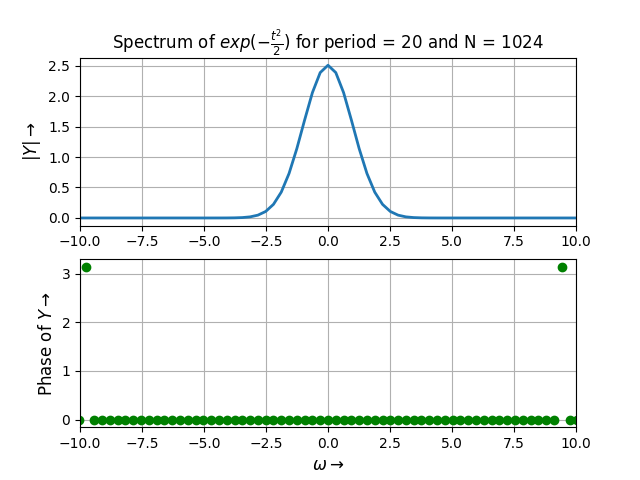
\includegraphics[scale = 0.8]{Figure_9.png}
    \label{fig:sample}
\end{figure}
\begin{center}
    This is the first period of the periodic repetition of the finite length signal ($T_{o} = 20$)
\end{center}
This new periodic function has a period of $T_{o}$ and hence a fundamental frequency of $\Omega_{0} = \frac{2\pi}{T_{o}}$. Hence the signal will have CTFS coefficients at frequencies which are multiples of $\Omega_{o}$. Now we have already proved in section (2.4) that:
\begin{equation*}
    X(k\Omega_{o}) = T_{o}a_{k}
\end{equation*}
and we know $X(\Omega)$ decreases as $\Omega$ increses. Hence we can safely say the CTFS coefficients are nearly 0 at high values of k. Now, the final step is to choose a sampling frequency such that we can safely assume the CTFT of this periodic signal is bandlimited within that range. Let's choose $N=1024$ and $T_{o} = 20$. Hence, $\Omega_{o} = \frac{2\pi}{T_{o}} = \frac{\pi}{10}$ and $\Omega_{s} = N\frac{2\pi}{T_{o}} = 1024\frac{\pi}{10}$. Clearly $\Omega_{s}$ is sufficiently high to assume that the Nyquist criteria is satisfied. \textbf{This is the second assumption}. With these two assumptions in mind, we can use all the results we got in section (2.4). The main result which we want is the following equation:
\begin{equation*}
    X(k\Omega_{o}) = T_{s}a[k]
\end{equation*}
Hence, whatever DFT coefficients vector we are getting, we need to multiply it by $T_{s}$. The resulting coefficients are nothing but the CTFT values of the windowed Gaussian signal at integral values of $\Omega_{o}$. The plot given below is for $T_{o} = 20$ and $N=1024$
\vspace*{-0.5cm}
\begin{figure}[H]
    \centering
    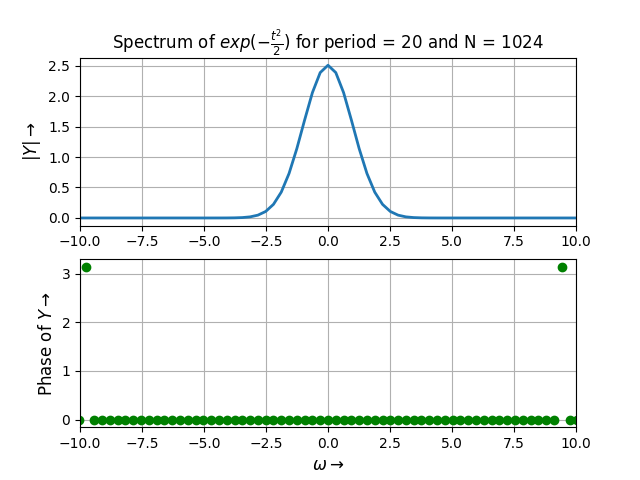
\includegraphics[scale = 0.8]{Figure_10.png}
    \label{fig:sample}
\end{figure}
\begin{center}
    The curve looks very much similar to the CTFT formula we derived
\end{center}
\subsection{Effect of $T_{o}$ and N on the CTFT of the Gaussian}
We already derived that the least count of CT frequency is $\Omega_{o} = \frac{2\pi}{T_{o}}$ and the frequency range is $[-\frac{\Omega_{s}}{2},\frac{\Omega_{s}}{2}) = [-N\frac{2\pi}{T_{o}},N\frac{2\pi}{T_{o}})$ 

With these facts in mind, let's understand the important pints to improve the spectrum plot of the Gaussian function:
\begin{enumerate}
    \item Increasing $T_{o}$ hase two benefits: 
    \begin{itemize}
        \item The window of the finite length signal iincreases and hence the approximation becomes more accurate. 
        \item The resolution improves and hence, the plot will be much more smoother.
    \end{itemize}
    \item Increasing N also has 2 benefits:
    \begin{itemize}
        \item The sampling frequency $\Omega_{s} = N\frac{2\pi}{T_{o}}$ increases and hence, the assumption that the Nyquist criteria is satisfied is much more credible
        \item We can get the CTFT for a broader range of frequency as the range is determined by N.
    \end{itemize}
\end{enumerate}

Hence we expect the graphs to become smoother with increase in period. Let's see if that's the case:

\begin{figure}[H]
    \centering
    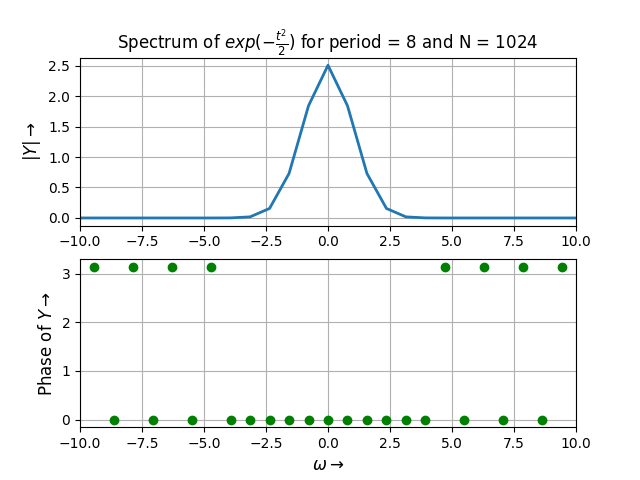
\includegraphics[scale = 0.8]{Figure_11.png}
    \label{fig:sample}
\end{figure}

\begin{figure}[H]
    \centering
    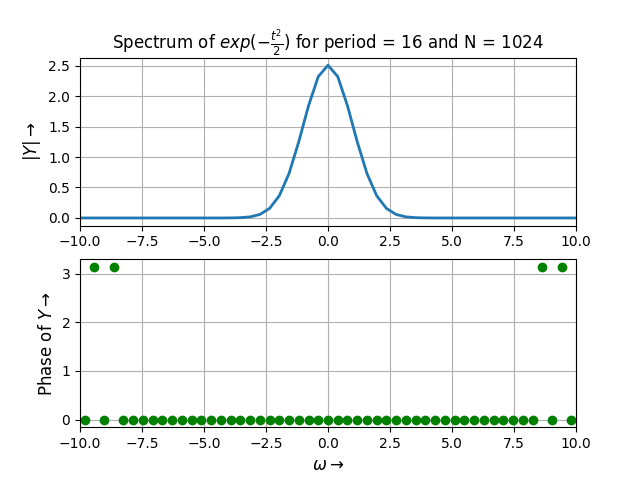
\includegraphics[scale = 0.8]{Figure_12.png}
    \label{fig:sample}
\end{figure}

\begin{figure}[H]
    \centering
    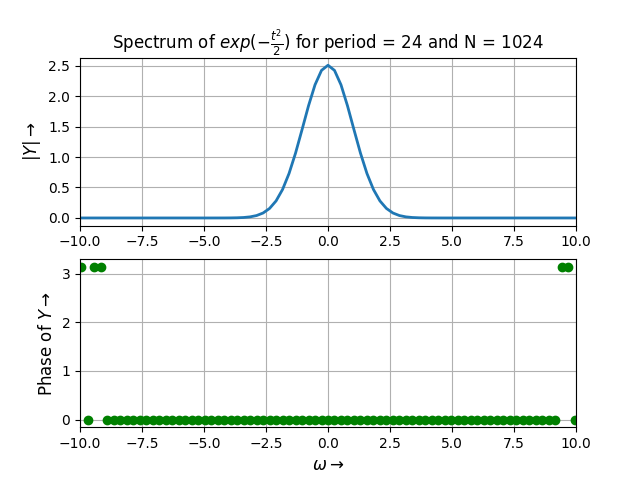
\includegraphics[scale = 0.8]{Figure_13.png}
    \label{fig:sample}
\end{figure}

\begin{figure}[H]
    \centering
    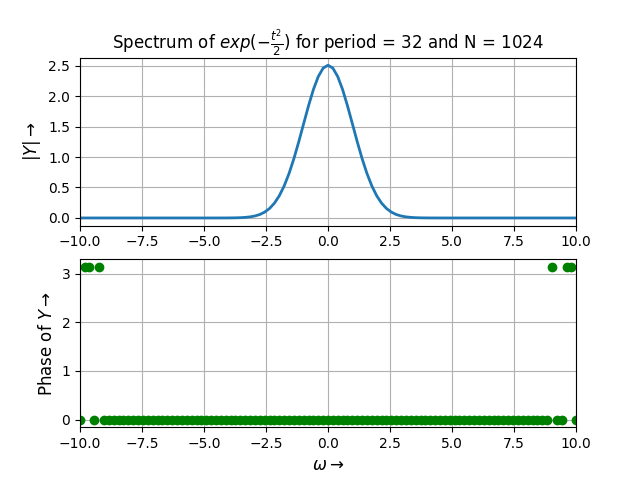
\includegraphics[scale = 0.8]{Figure_14.png}
    \label{fig:sample}
\end{figure}

\begin{figure}[H]
    \centering
    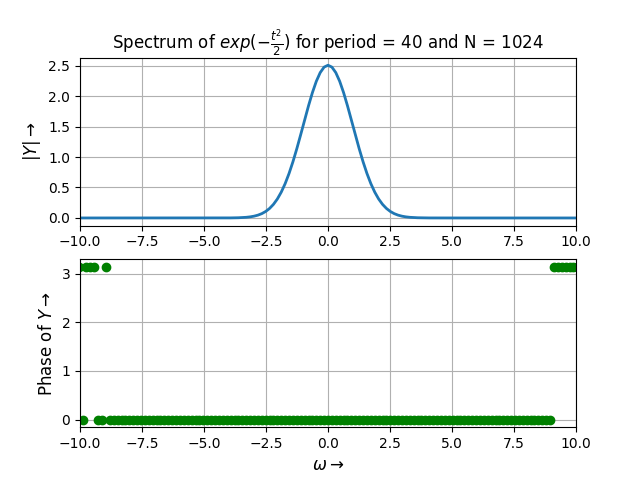
\includegraphics[scale = 0.8]{Figure_15.png}
    \label{fig:sample}
\end{figure}

Clearly the graph becomes smoother with increasing $T_{o}$ value. Also note that the maximum frequency range for which the CTFT is calculated is also decreasing because $\Omega_{s}$ inversely depends on $T_{o}$ for a given value of N. However in all the plots, the x-limit is set to $[-10,10)$. And the lowest frequency range in these set of plots is $\frac{\Omega_{s}}{2} = 512\frac{2\pi}{40} > 10$. Hence we aren't able to see the decreasing trend in the range of frequencies.


\textbf{Error plot:} As already said, whatever plots we are getting is an approximation and not the exact spectrum of the gaussian. That's why we are even getting phase values of $\pi$ at high frequencies (Could be due to computer precision or some other non-idealities). However, the graph we get is fairly accurate to the significant range of frequencies i.e., where the spectrum magnitude is more than 0.001. Now, let's see how the maximum error between the computed CTFT values and actual CTFT values change with the period. We expect a decreasing trend with increasing period as we have already seen higher period means better approximation. Let's see if the plot obeys this fact:
\begin{figure}[H]
    \centering
    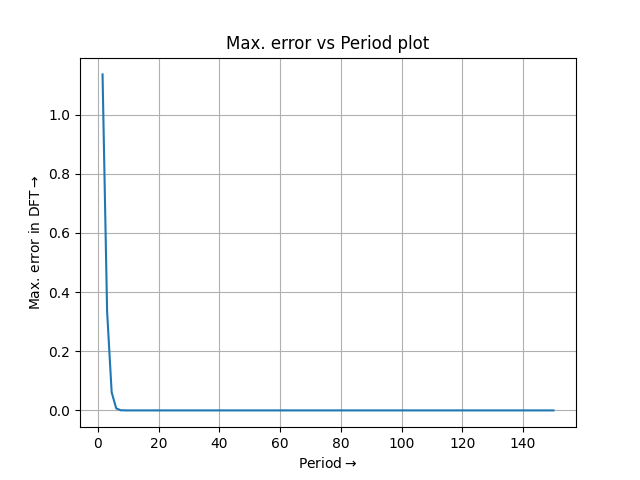
\includegraphics[scale = 0.8]{Figure_16.png}
    \label{fig:sample}
\end{figure}
\begin{center}
    In this example, the period $T_{o}$ starts from 1.5 and ranges till 150 in steps of 1.5. As expected, the error is decreasing with increasing $T_{o}$
\end{center}

\section{Conclusions}
\begin{enumerate}
    \item The spectrum plot of $\sin(5t)$ is exact and the CTFS coefficients are correctly computed.
    \item The spectrum plot of amplitude modulated signal is also exact. Only the resolution had to be improved to get an accurate plot.
    \item The spectra plots of $\sin^{3}(t)$ and $\cos^{3}(t)$ are also exact.
    \item The spectrum plot of frequency modulated signal is very much accurate when the chosen sampling frequency is sufficiently large and it exactly matched the Bessel's function plot generated manually.
    \item In all the above cases, the Nyquist criteria is satisfied and hence, the plots are exact.
    \item In the gaussian example, the CTFT spectrum plot obtained is very accurate when the window chosen is high because:
    \begin{itemize}
        \item High resolution
        \item Better approximation of the windowed signal with respect to the actual gaussian signal
    \end{itemize}
    \item To improve the resolution, the only method is to increase $T_{o}$. However, we can control the maximum frequency range (For which the CTFT is computed) by both N as well as $T_{o}$.
    \item The maximum error between the computed CTFT and actual CTFT decreases with increasing $T_{o}$ as expected.
    \item The window length $T_{o}$ must be choose so that the periodic repetition of the windowed gaussian almost mimics the sinusoid. In that case, the frequency components in the periodic signal would be less and hence the Nyquist criteria will also be satisfied much more accurately.
    \item However we have a trade-off here. Any increase in the period $T_{o}$ (ideal) will improve the approximation that the CTFT of the windowed signal is same as the CTFT of the original gaussian. However, now the periodic signal will have more frequency components and hence, the Nyquist criteria may not be obeyed fully. To resolve this issue, we must increase the value of N.
\end{enumerate}


\end{document}